\DiaryEntry{Bayesian Parameter Estimation - Disease Detection (2020-10-05, 2020-06-22)}{2019-02-22}{Stochastic}

A funny example from the book "Statistical Rethinking" (info \href{https://xcelab.net/rm/statistical-rethinking/}{here}).

Suppose we have a medical test which tests whether a person is ill or not. The test is no perfect; it yields a positive result when the tested person is ill with probability

\bee
P(pos. test | ill) = 0.9
\eee

and it returns a positive result when the person is healthy (a "false alarm") with probability

\bee
P(pos. test | healthy) = 0.1
\eee

Note that these two probabilities need not sum to one; however, $P(neg. test | ill) + P(pos. test | ill) = 1$.

In addition, we know that illness is very rare; this is modelled as

\bee
P(ill) = 0.001
\eee

We want to know the probability that a person is ill after she has received a positive test. This posterior probability is calculated using Bayes theorem as,

\begin{align*}
P(ill|pos. test) &= \frac{P(pos. test | ill) P(ill)}{P(pos. test)} \\ &= \frac{P(pos. test | ill) P(ill)}{P(pos. test|ill) P(ill) + P(pos. test | healthy) P(healthy)} \\ &= \frac{0.9 \cdot 0.001}{0.9 \cdot 0.001 + 0.1 \cdot 0.999} \approx 0.00893
\end{align*}

This is a pretty bad result - although the test is positive, it is highly unlikely that the person is ill!

In Statistical Rethinking (Chapter 3), a more intuitive view is presented: Assume we have a population of $100.000$ people. According to the prior, $100$ will be ill and $99.900$ are healthy. Of the $100$ ill persons, $90$ will have a positive test. Of the $99.900$ healthy people, $9.990$ will have a positive test.

The numbers of positive tests can be added (they are unrelated: one of them is the number of positive tests of ill people and the other the number of positive tests of healthy people); in total $10.080$ tests will be positive. So the probability that a person is ill and has a positive test is

\bee
P(ill|pos. test) = 90 / 10080 \approx 0.00893
\eee

This - of course - matches with the result from above. From the numbers above, it can be seen that the large false positive probability together with the low probability of being ill are ruining the test result.

We need to improve the test; the question is whether it is sufficient to improve $P(pos. test | ill)$, \emph{or} $P(pos. test | healthy)$, or \emph{both}?

Let's improve $P(pos. test | ill)$ first with $P(pos. test | ill) = 0.999$ and we obtain

\bee
P(ill|pos. test) = \frac{0.999 \cdot 0.001}{0.999 \cdot 0.001 + 0.1 \cdot 0.999} \approx 0.0099
\eee

Not really an improvement. Looking at the counts, we see that of the $100$ ill persons, $0.999 \times 100 = 99.9$ have a positive test; i.e. ``almost all''. However, nothing has changed on the large number of false positives and therefore the posterior probability is not much better.

Let's try improving $P(pos. test | healthy)$ instead and set $P(pos. test | healthy)=0.001$. Now we obtain

\bee
P(ill|pos. test) = \frac{0.9 \cdot 0.001}{0.9 \cdot 0.001 + 0.001 \cdot 0.999} \approx 0.474
\eee

Although the posterior probability increased, it is still a bad result; the result says if your test is positive, there is still only a 50-50 chance that your are ill. Looking at the counts, we see that from the $99.900$ healthy people, $99.900 \times 0.001 = 99.9$ will have a positive test. This is comparable to the positive tests of the people being actually ill and therefore the posterior probability approaches $1/2$.

It seems we need a better test with both $P(pos. test | ill)$ \emph{and} $P(pos. test | healthy)$ better. Let's combine the two previous values; i.e. $P(pos. test | ill) = 0.999$ and $P(pos. test | healthy)=0.001$ yields

\bee
P(ill|pos. test) = \frac{0.999 \cdot 0.001}{0.999 \cdot 0.001 + 0.001 \cdot 0.999} = 0.5
\eee

Still no improvement. It seems that $P(pos. test | healthy)$ must be below $P(ill)$ for the tests to be meaningful; let's go for $P(pos. test | healthy) = 0.0001$ and we obtain

\bee
P(ill|pos. test) = \frac{0.999 \cdot 0.001}{0.999 \cdot 0.001 + 0.0001 \cdot 0.999} = 0.909
\eee

which is a real improvement. From our $100$ ill peopole, $99.$ will have a positive test and from the $99.900$ healthy people, $99.900 \times 0.0001 \approx 10$ will have a positive test. The number of true positives is larger than the false positives and therefore the test becomes meaningful.

Let's analyse this in a bit more detail. If $P(pos. test | healthy) \rightarrow 0$, then $P(ill|pos. test) \rightarrow 1$. Interestingly, if $P(pos. test | ill) \rightarrow 1$, then

\bee
P(ill|pos. test) = \frac{P(ill)}{P(ill) + P(pos.test|healthy)P(healthy)}
\eee

and this does not necessarily approach $1$ (at least not until $P(pos.test|healthy) \rightarrow 0$). So, there is some fundamental asymmetry here. Assume that $P(ill) \ll 1$, we have $P(healthy) \approx 1$ and we get the following approximation,

\bee
P(ill|pos. test) \approx \frac{P(ill)}{P(ill) + P(pos.test|healthy)}
\eee

From this we see that for $P(ill|pos. test)$ to become large, $P(pos.test|healthy)$ must be (much) smaller than $P(ill)$. This is consistent with the ``count'' view from above, where the large number of false positives caused the tests to become meaningless. Even if the test is good with reasonable $P(pos.test|healthy)$, the large number of healthy people (caused by the illness being very rare) causes a high number of false positive people.

The following Figure shows a plot of $P(ill|pos. test)$ vs $P(pos.test|healthy)$ for different values of $P(pos.test|ill)$. It can be seen that $P(pos.test|healthy)$ must be smaller than $10^{-4} \approx P(ill)$ for $P(ill|pos. test)$ to reach $1$. In addition, the plot shows the small dependency of $P(ill|pos. test)$ on $P(pos.test|ill)$.

\begin{figure}[H]
    \centering
    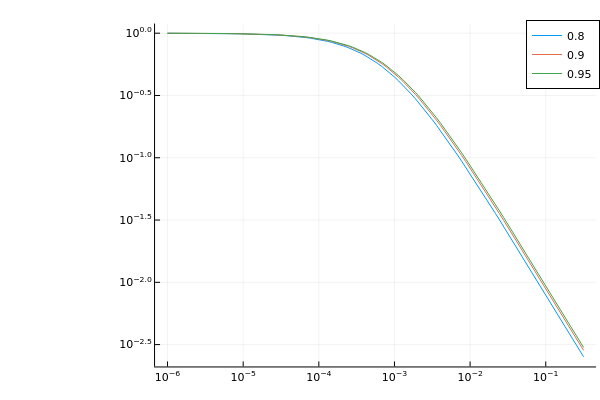
\includegraphics[scale=0.65]{images/bayes_illness_1.png}
\end{figure}

Things are much nicer if $P(ill)$ is larger; the following Figure shows similar plots as above for $P(ill)=0.1$. Notice the different parameter ranges and values!

\begin{figure}[H]
    \centering
    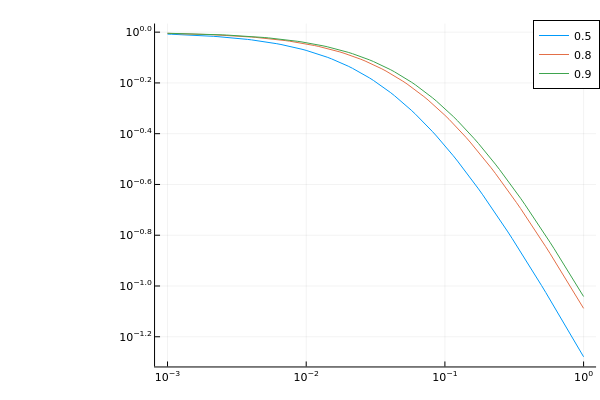
\includegraphics[scale=0.65]{images/bayes_illness_2.png}
\end{figure}



%%% Local Variables:
%%% mode: latex
%%% TeX-master: "journal"
%%% End:
